\section{The Lattice of Subgroups of a Group}

\begin{exercise}
    Let $H$ and $K$ be subgroups of $G$. Exhibit all possible sublattices which shows only $G$, 1, $H$, $K$ and their joins and intersections. What distinguishes the different drawings ? \\
\end{exercise}

\begin{solution}
    \\ To find these lattices, consider the three following cases : 
    \begin{enumerate}
        \item If $K \leq H$, then it obviously follows that $H \cap K = K$ and $\langle H,K \rangle = H$. Therefore, the lattice can be drawn as follows:
        
        \begin{center}
            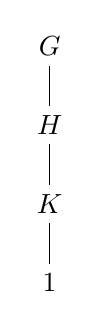
\begin{tikzpicture}
                %Nodes
                \node at (0,0) (G) {$G$};
                \node at (0,-1) (H) {$H$};
                \node at (0,-2) (K) {$K$};
                \node at (0,-3) (1) {$1$};
    
                %Lines
                \draw (1) -- (K);
                \draw (K) -- (H);
                \draw (H) -- (G);
            \end{tikzpicture}
        \end{center}

        \item If $H \leq K$, then it obviously follows that $H \cap K = H$ and $\langle H,K \rangle = K$. Therefore, the lattice can be drawn as follows:
        
        \begin{center}
            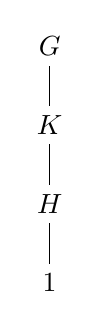
\begin{tikzpicture}
                %Nodes
                \node at (0,0) (G) {$G$};
                \node at (0,-1) (K) {$K$};
                \node at (0,-2) (H) {$H$};
                \node at (0,-3) (1) {$1$};
    
                %Lines
                \draw (1) -- (H);
                \draw (H) -- (K);
                \draw (K) -- (G);
            \end{tikzpicture}
        \end{center}

        \item If $H$ and $K$ are not comparable, all of $H$, $K$, $H\cap K$ and $\langle H,K \rangle$ are distinct. Hence:
        
        \begin{center}
            \begin{tikzpicture}
                %Nodes
                \node at (0,0)   (G)   {$G$};
                \node at (0,-1.5)(HUK) {$\langle H,K\rangle$};
                \node at (-2,-3) (H)   {$H$};
                \node at (2,-3)  (K)   {$K$};
                \node at (0,-4.5)(HAK){$H\cap K$};
                \node at (0,-6)  (1)   {$1$};
    
                %Lines
                \draw (1) -- (HAK);
                \draw (HAK) -- (H);
                \draw (HAK) -- (K);
                \draw (H) -- (HUK);
                \draw (K) -- (HUK);
                \draw (HUK) -- (G);
            \end{tikzpicture}
        \end{center}
    \end{enumerate}

    Therefore, the only thing that distinguishes the different drawings, beside the name of the nodes, is the fact that one is a straight line and the other splits in the middle. \\
\end{solution}

\begin{exercise}
    In each of (a) to (d) list all subgroups of $D_{16}$ that satisfy the given conition.
    \begin{enumerate}[label = \textbf{(\alph*)}]
        \item Subgroups that are contained in $\langle sr^2, r^4 \rangle$
        \item Subgroups that are contained in $\langle sr^7, r^4 \rangle$
        \item Subgroups that contain $\langle r^4 \rangle$
        \item Subgroups that contain $\langle s \rangle$.
    \end{enumerate}
\end{exercise}

\begin{solution}
    \begin{enumerate}[label = \textbf{(\alph*)}]
        \item The subgroups of $D_{16}$ that are contained in $\langle sr^2, r^4 \rangle$ are 
        $$1, \quad \langle sr^6\rangle, \quad \langle sr^2 \rangle, \quad \langle r^4 \rangle, \quad \langle sr^2, r^4 \rangle$$
        \item First, notice that $\langle sr^7, r^4 \rangle$ is equal to $\langle sr^3, r^4 \rangle$. Hence, the subgroups of $D_{16}$ that are contained in $\langle sr^7, r^4 \rangle$ are 
        $$1, \quad \langle sr^3\rangle, \quad \langle sr^7 \rangle, \quad \langle r^4 \rangle, \quad \langle sr^7, r^4 \rangle$$
        \item The subgroups of $D_{16}$ that contain $\langle r^4 \rangle$ are 
        $$\langle r^4 \rangle, \quad \langle sr^2, r^4\rangle, \quad \langle s, r^4\rangle, \quad \langle r^2\rangle, \quad \langle sr^3, r^4\rangle$$
        $$\langle sr^5, r^4\rangle, \quad \langle s, r^2\rangle, \quad \langle r \rangle, \quad \langle sr, r^2\rangle, \quad D_{16}$$
        \item The subgroups of $D_{16}$ that contain $\langle s \rangle$ are 
        $$\langle s \rangle, \quad \langle s, r^4\rangle, \quad \langle s, r^2\rangle, \quad D_{16}$$
    \end{enumerate}
\end{solution}

\begin{exercise}
    Show that the subgroup $\langle s, r^2\rangle$ of $D_8$ is isomorphic to $V_4$. \\
\end{exercise}

\begin{solution}
    \\ First, recall that $V_4 = \{1, a, b, c\}$ with the following multiplication table:

    \begin{table}[h!]
    \centering
    \begin{tabular}{l|l l l l}
    $\cdot$ & 1   & $a$ & $b$ & $c$ \\ \hline
    1       & 1   & $a$ & $b$ & $c$ \\ 
    $a$     & $a$ & 1   & $c$ & $b$ \\ 
    $b$     & $b$ & $c$ & 1   & $a$ \\ 
    $c$     & $c$ & $b$ & $a$ & 1  
    \end{tabular}
    \end{table}
    
    Notice that $\{1, s, r^2, sr^2\}$ is a group subgroup of $D_8$ that contains $s$, $r^2$ and all of the possible combinations of these elements. Hence,
    $$\langle s, r^2\rangle = \{1, s, r^2, sr^2\}$$
    From this, we get the following multiplication table for $\langle s, r^2\rangle$:

    \begin{table}[h!]
    \centering
    \begin{tabular}{l|l l l l}
    $\cdot$ & 1      & $s$    & $r^2$  & $sr^2$ \\ \hline
    1       & 1      & $s$    & $r^2$  & $sr^2$ \\ 
    $s$     & $s$    & 1      & $sr^2$ & $r^2$  \\ 
    $r^2$   & $r^2$  & $sr^2$ & 1      & $s$    \\ 
    $sr^2$  & $sr^2$ & $r^2$  & $s$    & 1  
    \end{tabular}
    \end{table}

    \break \noindent which directly implies that the function $\varphi : \langle s, r^2\rangle \to V_4$ defined by
    $$1 \mapsto 1, \quad a \mapsto s, \quad b \mapsto r^2, \quad c \mapsto sr^2$$
    is an isomorphism. Therefore, $\langle s, r^2\rangle \cong V_4$. \\
\end{solution}

\begin{exercise}
    Use the given lattice to find all pairs of elements that generate $D_8$ (there are 12 pairs). \\
\end{exercise}

\begin{solution}
    \\ Recall that the lattice of subgroups of $D_8$ looks like this:

    \begin{center}
        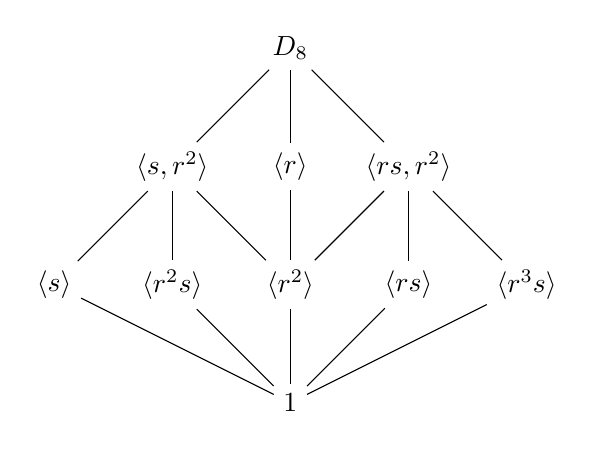
\begin{tikzpicture}
            %Nodes
            \node at (0,0)      (D8)  {$D_8$};
            \node at (0,-1.5)   (r)   {$\langle r \rangle$};
            \node at (-1.5,-1.5)(sr2){$\langle s,r^2\rangle$};
            \node at (1.5,-1.5) (rsr2){$\langle rs,r^2\rangle$};
            \node at (0,-3)     (r2)   {$\langle r^2 \rangle$};
            \node at (1.5,-3)   (rs)   {$\langle rs \rangle$};
            \node at (3,-3)     (r3s)  {$\langle r^3s \rangle$};
            \node at (-3,-3)    (s)  {$\langle s \rangle$};
            \node at (-1.5,-3)  (r2s) {$\langle r^2s \rangle$};
            \node at (0,-4.5)   (1){$1$};

            %Lines
            \draw (1)    -- (r2);
            \draw (1)    -- (r2s);
            \draw (1)    -- (s);
            \draw (1)    -- (rs);
            \draw (1)    -- (r3s);
            \draw (s)    -- (sr2);
            \draw (r2s)  -- (sr2);
            \draw (r2)   -- (sr2);
            \draw (r2)   -- (rsr2);
            \draw (rs)   -- (rsr2);
            \draw (r3s)  -- (rsr2);
            \draw (r2)   -- (r);
            \draw (sr2)  -- (D8);
            \draw (r)    -- (D8);
            \draw (rsr2) -- (D8);
        \end{tikzpicture}
    \end{center}
    Finding pairs $(a,b)$ such that $\langle a,b \rangle = D_8$ is equivalent to finding elements $a$ and $b$ such that the least common upperbound of their corresponding sets $\langle a \rangle$ and $\langle b \rangle$ on the lattice is $D_8$. Hence, if we recall that $\langle r^3 \rangle = \langle r \rangle$, then we get the following pairs:
    $$(s,r), \quad (s, rs), \quad (s,r^3s), \quad (r^2s,r), \quad (r^2s, rs), \quad (r^2s,r^3s)$$
    $$(s,r^3), \quad (r, rs), \quad (r,r^3s), \quad (r^2s,r^3), \quad (r^3, rs), \quad (r^3,r^3s)$$
    \break
\end{solution}

\begin{exercise}
    Use the given lattice to find all elements $x \in D_{16}$ such that $D_{14} = \langle x, s \rangle$ (there are 8 such elements). \\
\end{exercise}

\begin{solution}
    \\ The idea is exactly the same as for the previous exercise. Hence, our possible values for $x$ are:
    $$r, \quad r^3, \quad r^5, \quad r^7, \quad sr, \quad sr^3, \quad sr^5, \quad sr^7$$
\end{solution}

\begin{exercise}
    Use the given lattices to help find the centralizers of every element in the following groups:\\
    $\textbf{(a)} \ D_8 \qquad \textbf{(b)} \ Q_8 \qquad \textbf{(c)} \ S_3 \qquad \textbf{(d)} \ D_{16} $ \\
\end{exercise}

\begin{solution}
    \begin{enumerate}[label = \textbf{(\alph*)}]
        \item \begin{multicols}{3}\begin{itemize}
            \item $C_{D_8}(1) = D_8$
            \item $C_{D_8}(r) = \langle r \rangle$
            \item $C_{D_8}(r^2) = D_8$
            \item $C_{D_8}(r^3) = \langle r \rangle$
            \item $C_{D_8}(s) = \langle s, r^2 \rangle$
            \item $C_{D_8}(rs) = \langle rs, r^2 \rangle$
            \item $C_{D_8}(r^2s) = \langle s, r^2 \rangle$
            \item $C_{D_8}(r^3s) = \langle rs, r^2 \rangle$
        \end{itemize}
        \end{multicols}
        \item \begin{multicols}{3}\begin{itemize}
            \item $C_{Q_8}(1) = Q_8$
            \item $C_{Q_8}(-1) = Q_8$
            \item $C_{Q_8}(i) = \langle i \rangle$
            \item $C_{Q_8}(-i) = \langle i \rangle$
            \item $C_{Q_8}(j) = \langle j \rangle$
            \item $C_{Q_8}(-j) = \langle j \rangle$
            \item $C_{Q_8}(k) = \langle k \rangle$
            \item $C_{Q_8}(-k) = \langle k \rangle$
        \end{itemize}
        \end{multicols}
    \item \begin{multicols}{2}\begin{itemize}
            \item $C_{S_3}(1) = S_3$
            \item $C_{S_3}((1 \ 2)) = \langle (1 \ 2) \rangle$
            \item $C_{S_3}((1 \ 3)) = \langle (1 \ 3) \rangle$
            \item $C_{S_3}((2 \ 3)) = \langle (2 \ 3) \rangle$
            \item $C_{S_3}((1 \ 2 \ 3)) = \langle (1 \ 2 \ 3) \rangle$
            \item $C_{S_3}((1 \ 3 \ 2)) = \langle (1 \ 3 \ 2) \rangle$
        \end{itemize}
        \end{multicols}
    \item \begin{multicols}{2}\begin{itemize}
            \item $C_{D_{16}}(1) = D_{16}$
            \item $C_{D_{16}}(r) = \langle r \rangle$
            \item $C_{D_{16}}(r^2) = \langle r \rangle$
            \item $C_{D_{16}}(r^3) = \langle r \rangle$
            \item $C_{D_{16}}(r^4) = D_{16}$
            \item $C_{D_{16}}(r^5) = \langle r \rangle$
            \item $C_{D_{16}}(r^6) = \langle r \rangle$
            \item $C_{D_{16}}(r^7) = \langle r \rangle$
            \item $C_{D_{16}}(s) = \langle s, r^4 \rangle$
            \item $C_{D_{16}}(sr) = \langle sr^5, r^4 \rangle$
            \item $C_{D_{16}}(sr^2) = \langle sr^2, r^4 \rangle$
            \item $C_{D_{16}}(sr^3) = \langle sr^3, r^4 \rangle$
            \item $C_{D_{16}}(sr^4) = \langle s, r^4 \rangle$
            \item $C_{D_{16}}(sr^5) = \langle sr^5, r^4 \rangle$
            \item $C_{D_{16}}(sr^6) = \langle sr^2, r^4 \rangle$
            \item $C_{D_{16}}(sr^7) = \langle sr^3, r^4 \rangle$
        \end{itemize}
        \end{multicols}
    \end{enumerate}
\end{solution}

\begin{exercise}
    Find the center of $D_{16}$.\\
\end{exercise}

\begin{solution}
    \\ To find the center of $D_{16}$, we can take the intersection of all the subgroups we found in part (d) of the previous question, that is:
    $$D_{16}\cap \langle r \rangle \cap \langle s, r^4 \rangle \cap \langle sr^2, r^4 \rangle \cap \langle sr^3, r^4 \rangle \cap \langle sr^5, r^4 \rangle$$
    Obviously, 1 and $r^4$ are in this intersection. However, since $sr^i \notin \langle r \rangle$ for $i \in \Iint{0}{n-1}$, then other elements in the intersection must be powers of $r$. However, the only power of $r$ in $\langle s, r^4 \rangle$ is $r^4$. Therefore,
    $$Z(D_{16}) = \{1, r^4\}$$
\end{solution}

\begin{exercise}
    In each of the following groups find the normalizer of each subgroup:\\
    $\textbf{(a)} \ S_3 \qquad \textbf{(b)} \ Q_8$ \\
\end{exercise}

\begin{solution}
    \begin{enumerate}[label = \textbf{(\alph*)}]
        \item \begin{multicols}{2}\begin{itemize}
            \item $N_{S_3}(1) = S_3$
            \item $N_{S_3}(\langle (1 \ 2) \rangle) = \langle (1 \ 2) \rangle$
            \item $N_{S_3}(\langle (1 \ 3) \rangle) = \langle (1 \ 3) \rangle$
            \item $N_{S_3}(\langle (2 \ 3) \rangle) = \langle (2 \ 3) \rangle$
            \item $N_{S_3}(\langle (1 \ 2 \ 3) \rangle) = S_3$
            \item $N_{S_3}(S_3) = S_3$
        \end{itemize}
        \end{multicols}
        \item \begin{multicols}{2}\begin{itemize}
            \item $N_{Q_8}(1) = Q_8$
            \item $N_{Q_8}(\langle -1 \rangle) = Q_8$
            \item $N_{Q_8}(\langle i \rangle) = Q_8$
            \item $N_{Q_8}(\langle j \rangle) = Q_8$
            \item $N_{Q_8}(\langle k \rangle) = Q_8$
            \item $N_{Q_8}(Q_8) = Q_8$
        \end{itemize}
        \end{multicols}
    \end{enumerate}
\end{solution}

\begin{exercise}
    Draw the lattices of subrgoups of the following groups:\\
    $\textbf{(a)} \ \Z{16} \qquad \textbf{(b)} \ \Z{24} \qquad \textbf{(c)} \ \Z{48}. \ $ [See Exercise 6 in Section 3.]\\ 
\end{exercise}

\begin{solution}
    \begin{enumerate}[label = \textbf{(\alph*)}]
        \item Lattice of subgroups of $\Z{16}$:
            \begin{center}
            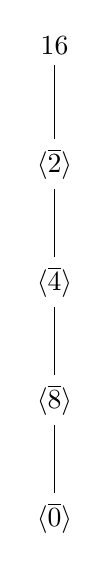
\begin{tikzpicture}
                %Nodes
                \node at (0,0)      (1)  {$\Z{16}$};
                \node at (0,-1.5)   (2)  {$\langle \overline{2} \rangle$};
                \node at (0,-3)     (4)  {$\langle \overline{4} \rangle$};
                \node at (0,-4.5)   (8)  {$\langle \overline{8} \rangle$};
                \node at (0,-6)     (0) {$\langle \overline{0} \rangle$};
    
    
                %Lines
                \draw (1) -- (2);
                \draw (2) -- (4);
                \draw (4) -- (8);
                \draw (8) -- (0);
            \end{tikzpicture}
            \end{center}
        \item Lattice of subgroups of $\Z{24}$:
            \begin{center}
            \begin{tikzpicture}
                %Nodes
                \node at (1.5,0)   (1)  {$\Z{24}$};
                \node at (0,-1.5)  (3)  {$\langle \overline{3} \rangle$};
                \node at (3,-1.5)  (2)  {$\langle \overline{2} \rangle$};
                \node at (1.5,-3)  (6)  {$\langle \overline{6} \rangle$};
                \node at (4.5,-3)  (4)  {$\langle \overline{4} \rangle$};
                \node at (3,-4.5)  (12) {$\langle \overline{12} \rangle$};
                \node at (6,-4.5)  (8)  {$\langle \overline{8} \rangle$};
                \node at (4.5,-6)  (0) {$\langle \overline{0} \rangle$};
    
    
                %Lines
                \draw (1) -- (3);
                \draw (1) -- (2);
                \draw (6) -- (2);
                \draw (3) -- (6);
                \draw (6) -- (12);
                \draw (2) -- (4);
                \draw (4) -- (12);
                \draw (12) -- (0);
                \draw (4) -- (8);
                \draw (8) -- (0);
            \end{tikzpicture}
            \end{center}
        \item We already drew the lattice of subgroups of $\Z{48}$ in Exercise 6 of section 3:
        \begin{center}
            \begin{tikzpicture}
                %Nodes
                \node at (1.5,0)   (1)  {$\mathbb{Z}/48\mathbb{Z}$};
                \node at (0,-1.5)  (3)  {$\langle \overline{3} \rangle$};
                \node at (3,-1.5)  (2)  {$\langle \overline{2} \rangle$};
                \node at (1.5,-3)  (6)  {$\langle \overline{6} \rangle$};
                \node at (4.5,-3)  (4)  {$\langle \overline{4} \rangle$};
                \node at (3,-4.5)  (12) {$\langle \overline{12} \rangle$};
                \node at (6,-4.5)  (8)  {$\langle \overline{8} \rangle$};
                \node at (4.5,-6)  (24) {$\langle \overline{24} \rangle$};
                \node at (7.5,-6)  (16) {$\langle \overline{16} \rangle$};
                \node at (6,-7.5)  (0)  {$\langle \overline{0} \rangle$};
    
    
                %Lines
                \draw (1) -- (3);
                \draw (1) -- (2);
                \draw (6) -- (2);
                \draw (3) -- (6);
                \draw (6) -- (12);
                \draw (2) -- (4);
                \draw (4) -- (12);
                \draw (12) -- (24);
                \draw (4) -- (8);
                \draw (8) -- (24);
                \draw (0) -- (24);
                \draw (8) -- (16);
                \draw (0) -- (16);
            \end{tikzpicture}
        \end{center}
    \end{enumerate}
\end{solution}

\begin{exercise}
    Classify groups of order 4 by proving that if $|G|=4$ then $G \cong Z_4$ or $G \cong V_4$. [See Exercise 36, Section 1.1.] \\
\end{exercise}

\begin{solution}
    \\ Let's prove it by cases. If $G$ contains an element of order 4, then it directly follows that $G$ is a cyclic group of order 4 which implies that $G \cong Z_4$. \\
    Otherwise, if $G$ has no elements of order 4, then we already proved in Exercise 36 of Section 1.1 that it automoaticaly implies that $G$ has the following multiplication table:
    \begin{table}[h!]
        \centering
        \begin{tabular}{l|l l l l}
        $\cdot$ & 1   & $a$ & $b$ & $c$ \\ \hline
        1       & 1   & $a$ & $b$ & $c$ \\ 
        $a$     & $a$ & 1   & $c$ & $b$ \\ 
        $b$     & $b$ & $c$ & 1   & $a$ \\ 
        $c$     & $c$ & $b$ & $a$ & 1  
        \end{tabular}
    \end{table}
    which is exactly the same multiplication as $V_4$ so both are isomorphic. Therefore, we either have $G \cong Z_4$ or $G \cong V_4$. \\
\end{solution}

\begin{exercise}
    Consider the group of order 16 with the following presentation:
    $$QD_{16} = \langle \ \sigma, \tau \ | \ \sigma^8 = \tau^2 = 1, \ \sigma\tau = \tau\sigma^3 \ \rangle$$
    (called the \textit{quasidihedral} or \textit{semidihedral} group of order 16). This group has three subgroups of order 8: $\langle \tau, \sigma^2 \rangle \cong D_8$, $\langle \tau \rangle \cong Z_8$ and $\langle \sigma^2, \sigma\tau \rangle \cong Q_8$ and every proper subgroup is contained in one of these subgroups. Fill in the missing subgroups in the lattice of all subgroups of the quasidihedral group on the following page, exhibiting each subgroup with at most two generators. (This is another example of a nonplanar lattice.) \\
\end{exercise}

\begin{solution}
    \\ Using the isomorphisms $\langle \tau, \sigma^2 \rangle \cong D_8$, $\langle \tau \rangle \cong Z_8$ and $\langle \sigma^2, \sigma\tau \rangle \cong Q_8$, we can make our life easier by considering $\sigma^2$ and $\tau$ as $r$ and $s$ respectively in $D_8$. Moreover, in the same way, we can consider $\sigma^4$, $\sigma^2$, $\tau\sigma$ and $\tau\sigma^7$ as -1, $i$, $j$ and $k$ respectively. Therefore, we get the following lattice of subgroups for $QD_{16}$:
    \begin{center}
        \begin{tikzpicture}
            %Nodes
            \node at (0,0)   (16)    {$QD_{16}$};
            \node at (-3,-2.5) (s2t)  {$\langle \sigma^2, \tau \rangle$}; 
            \node at (0,-2.5)  (s)    {$\langle \sigma \rangle$}; 
            \node at (3,-2.5) (s2ts)  {$\langle \sigma^2, \tau\sigma \rangle$};
            \node at (-6,-5)  (s2ts4) {$\langle \sigma^2\tau, \sigma^4 \rangle$};
            \node at (-3,-5)  (s4t) {$\langle \sigma^4, \tau \rangle$}; 
            \node at (0,-5)   (s2)  {$\langle \sigma^2 \rangle$};
            \node at (3,-5)   (ts)  {$\langle \tau \sigma \rangle$};
            \node at (6,-5)   (ts7)  {$\langle \tau \sigma^7 \rangle$};
            \node at (-7,-7.5) (ts2)  {$\langle \tau \sigma^2 \rangle$};
            \node at (-5,-7.5) (s2th)  {$\langle \sigma^2 \tau\rangle$};
            \node at (-3.5,-7.5) (s4th)  {$\langle \sigma^4 \tau\rangle$};
            \node at (-2,-7.5) (t)  {$\langle \tau \rangle$};
            \node at (0,-7.5) (s4)  {$\langle \sigma^4 \rangle$};
            \node at (0,-10) (1)  {1};
            \node (i) at (intersection of s4--s2ts4 and s4t--s4th) {}; 
            \node (ii) at (intersection of s4--s2ts4 and s4t--t) {}; 

            %Lines
            \draw (16) -- (s2t);
            \draw (16) -- (s);
            \draw (16) -- (s2ts);
            \draw (s2t) -- (s2ts4);
            \draw (s2t) -- (s4t);
            \draw (s2t) -- (s2);
            \draw (s) -- (s2);
            \draw (s2ts) -- (s2);
            \draw (s2ts) -- (ts);
            \draw (s2ts) -- (ts7);
            \draw (ts2) -- (s2ts4);
            \draw (s2th) -- (s2ts4);
            \draw (s4th) -- (i);
            \draw (i) -- (s4t);
            \draw (t) -- (ii);
            \draw (ii) -- (s4t);
            \draw (s4) -- (s4t);
            \draw (s4) -- (s2);
            \draw (s4) -- (ts);
            \draw (s4) -- (ts7);
            \draw (s4) -- (s2ts4);
            \draw (1) -- (ts2);
            \draw (1) -- (s2th);
            \draw (1) -- (s4th);
            \draw (1) -- (t);
            \draw (1) -- (s4);
        \end{tikzpicture}
    \end{center}
\end{solution}

\begin{exercise}
    The group $A = Z_2 \times Z_4 = \langle \ a,b \ | a^2 = b^4 = 1, \ ab = ba \ \rangle$ has order 8 and has three subgroups of order 4: $\langle a, b^2 \rangle \cong V_4$, $\langle b \rangle \cong Z_4$ and $\langle a b \rangle \cong Z_4$ and every proper subgroup is contained in one of these three. Draw the lattice of all subgroups of $A$, giving each subgroup in terms of at most two generators. \\
\end{exercise}

\begin{solution}
    As in the previous exercise, we will mostly rely on the fact that all the subgroups of order 4 are $\langle a, b^2 \rangle \cong V_4$, $\langle b \rangle \cong Z_4$ and $\langle a b \rangle \cong Z_4$. Hence, we get:
    \begin{center}
        \begin{tikzpicture}
            %Nodes
            \node at (0,0)   (A)    {$A$};
            \node at (-3,-2) (ab2)  {$\langle a,b^2\rangle$}; 
            \node at (0,-2)  (b)    {$\langle b \rangle$}; 
            \node at (3,-2)  (ab)   {$\langle ab \rangle$};
            \node at (-6,-4) (a)    {$\langle a \rangle$};
            \node at (-3,-4) (ab2h) {$\langle ab^2 \rangle$}; 
            \node at (0,-4)  (b2)   {$\langle b^2 \rangle$};
            \node at (0,-6)  (1)    {$ 1 $};

            %Lines
            \draw (A) -- (ab2);
            \draw (A) -- (b);
            \draw (A) -- (ab);
            \draw (a) -- (ab2);
            \draw (ab2h) -- (ab2);
            \draw (b2) -- (ab2);
            \draw (b2) -- (b);
            \draw (b2) -- (ab);
            \draw (a) -- (1);
            \draw (ab2h) -- (1);
            \draw (b2) -- (1);
        \end{tikzpicture}
    \end{center}
\end{solution}

\begin{exercise}
    The group $G = Z_2 \times Z_8 = \langle \ x,y \ | x^2 = y^8 = 1, \ xy = yx \ \rangle$ has order 16 and has three subgroups of order 8: $\langle x, y^2 \rangle \cong Z_2\times Z_4$, $\langle y \rangle \cong Z_8$ and $\langle xy \rangle \cong Z_8$ and every proper subgroup is contained in one of these three. Draw the lattice of all subgroups of $G$, giving each subgroup in terms of at most two generators (cf. Exercise 12 ). \\
\end{exercise}

\begin{solution}
    As in the previous exercise, we will mostly rely on the fact that all the subgroups of order 8 are $\langle x, y^2 \rangle \cong Z_2\times Z_4$, $\langle y \rangle \cong Z_8$ and $\langle xy \rangle \cong Z_8$. Moreover, since we already drew the lattice of subgroups of the group $Z_2 \times Z_4$ in the previous question, then we get:
    \begin{center}
        \begin{tikzpicture}
            %Nodes
            \node at (0,0)   (G)    {$G$};
            \node at (-3,-2) (y)   {$\langle y \rangle$}; 
            \node at (0,-2)  (xy)    {$\langle xy \rangle$}; 
            \node at (3,-2)  (xvy2) {$\langle x,y^2 \rangle$};
            \node at (0,-4) (y2)   {$\langle y^2 \rangle$}; 
            \node at (3,-4)  (xy2)  {$\langle xy^2 \rangle$};
            \node at (6,-4)  (xvy4) {$\langle x,y^4 \rangle$};
            \node at (3,-6) (y4)   {$\langle y^4 \rangle$}; 
            \node at (6,-6)  (x)    {$\langle x \rangle$};
            \node at (9,-6)  (xy4)  {$\langle xy^4 \rangle$};
            \node (i) at (intersection of y4--xvy4 and x--xy2) {}; 
            \node at (6,-8)  (1)    {$ 1 $};

            %Lines
            \draw (G) -- (xy);
            \draw (G) -- (y);
            \draw (G) -- (xvy2);
            \draw (y2) -- (xy);
            \draw (y2) -- (y);
            \draw (y2) -- (xvy2);
            \draw (xy2) -- (xvy2);
            \draw (xvy4) -- (xvy2);
            \draw (y4) -- (y2);
            \draw (y4) -- (xy2);
            \draw (y4) -- (i);
            \draw (i) -- (xvy4);
            \draw (x) -- (xy2);
            \draw (xy4) -- (xvy4);
            \draw (y4) -- (1);
            \draw (x) -- (1);
            \draw (x) -- (xvy4);
            \draw (xy4) -- (1);
        \end{tikzpicture}
    \end{center}
\end{solution}

\begin{exercise}
    Let $M$ be the group of order 16 with the following presentation:
    $$\langle \ u,v \ | \ u^2 = v^8 = 1, \ vu = uv^5 \ \rangle$$
    (sometimes called the \textit{modular} group of order 16). It has three subgroups of order 8: $\langle u,v^2 \rangle$, $\langle v \rangle$ and $\langle uv \rangle$ and every proper subgroup is contained in oneof these three. Prove that $\langle u, v^2 \rangle \cong Z_2\times Z_4$, $\langle v \rangle \cong Z_8$ and $\langle uv \rangle \cong Z_8$. Show that the lattice of subgroups of $M$ is the same as the lattice of subgroups of $Z_2 \times Z_8$ (cf. Exercise 13) but that these two groups are not isomorphic. \\
\end{exercise}

\begin{solution}
    \\ First, let's prove the three isomorphisms. Obviously, $\langle v \rangle \cong Z_8$ since $v$ is an element of order 8. Similarly, to show that $\langle uv \rangle \cong Z_8$, we simply need to show that $uv$ has order 8. To do so, notice that 
    $$(uv)^2 = uvuv = uuv^5v = v^6$$
    Thus,
    $$(uv)^8 = (v^6)^4 = v^{24} = 1$$
    Hence, $uv$ must have order 1, 2, 4 or 8. But notice that
    $$(uv)^4 = (v^6)^2 = v^12 = v^4 \neq 1$$
    Therefore, $uv$ has order 8 which shows that $\langle uv \rangle \cong Z_8$. Finally, since
    $$uv^2 = (uv^2)v^8 = (uv^5)v^5 = v(uv^5) = v^2u$$
    then elements in $\langle u, v^2 \rangle$ have the form $u^n(v^2)^m$. Thus, obviously, $\langle u, v^2 \rangle \cong Z_2\times Z_4$. From this, we get that
    \begin{center}
        \begin{tikzpicture}
            %Nodes
            \node at (0,0)   (G)    {$G$};
            \node at (-3,-2) (y)   {$\langle v \rangle$}; 
            \node at (0,-2)  (xy)    {$\langle uv \rangle$}; 
            \node at (3,-2)  (xvy2) {$\langle u,v^2 \rangle$};
            \node at (0,-4) (y2)   {$\langle v^2 \rangle$}; 
            \node at (3,-4)  (xy2)  {$\langle uv^2 \rangle$};
            \node at (6,-4)  (xvy4) {$\langle u,v^4 \rangle$};
            \node at (3,-6) (y4)   {$\langle v^4 \rangle$}; 
            \node at (6,-6)  (x)    {$\langle u \rangle$};
            \node at (9,-6)  (xy4)  {$\langle uv^4 \rangle$};
            \node (i) at (intersection of y4--xvy4 and x--xy2) {}; 
            \node at (6,-8)  (1)    {$ 1 $};

            %Lines
            \draw (G) -- (xy);
            \draw (G) -- (y);
            \draw (G) -- (xvy2);
            \draw (y2) -- (xy);
            \draw (y2) -- (y);
            \draw (y2) -- (xvy2);
            \draw (xy2) -- (xvy2);
            \draw (xvy4) -- (xvy2);
            \draw (y4) -- (y2);
            \draw (y4) -- (xy2);
            \draw (y4) -- (i);
            \draw (i) -- (xvy4);
            \draw (x) -- (xy2);
            \draw (xy4) -- (xvy4);
            \draw (y4) -- (1);
            \draw (x) -- (1);
            \draw (x) -- (xvy4);
            \draw (xy4) -- (1);
        \end{tikzpicture}
    \end{center}
    which obviously shows that $M$ has the same lattice of subgroups of $Z_2 \times Z_8$.\\
    Now, let's show that $M \not\cong Z_2 \times Z_8$. By contradiction, if $M \cong Z_2 \times Z_8$, then $M$ must be abelian so we have 
    $$uv = vu = uv^5$$
    which implies that 
    $$v^4 = 1$$
    But this is a contradiction since $v$ has order 8. Therefore, $M \not\cong Z_2 \times Z_8$ even if they have the same lattice of subgroups. \\
\end{solution}

\begin{exercise}
    Describe the isomorphism type of each of the three subgroups of $D_{16}$ of order 8. \\
\end{exercise}

\begin{solution}
    The three subgroups of order 8 of $D_{16}$ are $\langle s, r^2 \rangle$, $\langle r \rangle$ and $\langle sr, r^2 \rangle$. Obviously, $\langle r \rangle \cong Z_8$ since it is cyclic and has order 8. By looking at the lattice of subgroups of $D_{16}$ and $D_8$, we can guess that both $\langle s, r^2 \rangle$ and $\langle sr, r^2 \rangle$ are isomorphic to $D_8$. To prove it, notice that the function that associates $s$ in $D_{16}$ to $s$ in $D_8$ and $r^2$ in $D_{16}$ to $r$ in $D_8$ extends to an isomorphism since $s$ has order 2, $r^2$ has order 4 and 
    $$(r^2)s = r(rs) = (rs)r^{-1} = s(r^2)^{-1}$$
    The same holds if we replace $s$ with $sr$. Therefore, we get that $\langle s, r^2 \rangle \cong \langle sr, r^2 \rangle \cong D_8$. \\
\end{solution}

\begin{exercise}
    Use the lattice of subgroups of the quasidihedral group of order 16 to show that every element of order 2 is contained in the proper subgroup $\langle \tau, \sigma^2 \rangle$ (cf. Exercise 11). \\
\end{exercise}

\begin{solution}
    \\ Proving this is equivalent to showing that every subgroup of $QD_{16}$ of order 2 is a subgroup of $\langle \tau, \sigma^2 \rangle$. The subgroups of order 2 are precisely $\langle \tau \rangle$, $\langle \sigma^4 \rangle$, $\langle \sigma^4\tau \rangle$, $\langle \sigma^2\tau \rangle$ and $\langle \tau\sigma^2 \rangle$. But notice that all of them are \textit{below} $\langle \tau, \sigma^2 \rangle$ in the lattice. Thus, $\langle \tau, \sigma^2 \rangle$ contains every element of order 2. \\
\end{solution}

\begin{exercise}
    Use the lattice of subgroups of the modular group $M$ of order 16 to show that the set $\{x\in M \ | \ x^2 = 1\}$ is a subgroup of $M$ isomorphic to the Klein 4-group (cf. Exercise 14). \\
\end{exercise}

\begin{solution}
    \\ The elements $x$ in $M$ that satisfy $x^2 = 1$ are precisely 1, $v^4$, $u$ and $uv^4$. But notice that $\langle u, v^4 \rangle$ contains exactly these four elements. Hence, it is a subgroup of $M$ of order 4 that is not cyclic, thus, it must isomorphic the Klein 4-group. \\ 
\end{solution}

\begin{exercise}
    Use the lattice to help find the centralizers of every element of $QD_{16}$ (cf. Exercise 11). \\
\end{exercise}

\begin{solution}
    \begin{multicols}{2}\begin{itemize}
        \item $C_{QD_{16}}(1) = QD_{16}$
        \item $C_{QD_{16}}(\sigma) = \langle \sigma \rangle$
        \item $C_{QD_{16}}(\sigma^2) = \langle \sigma \rangle$
        \item $C_{QD_{16}}(\sigma^3) = \langle \sigma \rangle$
        \item $C_{QD_{16}}(\sigma^4) = QD_{16}$
        \item $C_{QD_{16}}(\sigma^5) = \langle \sigma \rangle$
        \item $C_{QD_{16}}(\sigma^6) = \langle \sigma \rangle$
        \item $C_{QD_{16}}(\sigma^7) = \langle \sigma \rangle$
        \item $C_{QD_{16}}(\tau) = \langle \sigma^4, \tau \rangle$
        \item $C_{QD_{16}}(\tau\sigma) = \langle \tau\sigma \rangle$
        \item $C_{QD_{16}}(\tau\sigma^2) = \langle \sigma^2\tau, \sigma^4 \rangle$
        \item $C_{QD_{16}}(\tau\sigma^3) = \langle \tau \sigma^7 \rangle$
        \item $C_{QD_{16}}(\tau\sigma^4) = \langle \sigma^4, \tau \rangle$
        \item $C_{QD_{16}}(\tau\sigma^5) = \langle \tau\sigma \rangle$
        \item $C_{QD_{16}}(\tau\sigma^6) = \langle \sigma^2\tau, \sigma^4 \rangle$
        \item $C_{QD_{16}}(\tau\sigma^7) = \langle \tau\sigma^7 \rangle$
    \end{itemize}
    \end{multicols}
\end{solution}

\begin{exercise}
    Use the lattice to help find $N_{D_{16}}(\langle s, r^4 \rangle)$.\\
\end{exercise}

\begin{solution}
    \\ To find the normalizer of $\langle s, r^4 \rangle$, first notice that 
    \begin{align*}
        s\langle s, r^4 \rangle s^{-1} &= \{s1s, \ sss, \ sr^4s, \ ssr^4s\} \\
        &= \{1, \ s, \ r^4, \ sr^4\} \\
        &= \langle s, r^4 \rangle
    \end{align*}
    and 
    \begin{align*}
        r^2\langle s, r^4 \rangle r^{-2} &= \{r^2 1r^{-2}, \ r^2 sr^{-2}, \ r^2 r^4 r^{-2}, \ r^2 sr^4 r^{-2}\} \\
        &= \{1, \ sr^4, \ r^4, \ s\} \\
        &= \langle s, r^4 \rangle
    \end{align*}
    which implies that both $s$ and $r^2$ are in $N_{D_{16}}(\langle s, r^4 \rangle)$. Thus, $\langle s, r^2 \rangle \leq N_{D_{16}}(\langle s, r^4 \rangle)$ which implies by the given lattice that $N_{D_{16}}(\langle s, r^4 \rangle)$ is either $\langle s, r^2 \rangle$ or $D_{16}$. However, notice that 
    \begin{align*}
        r\langle s, r^4 \rangle r^{-1} &= \{r 1 r^{-1}, \ r sr^{-1}, \ r r^4 r^{-1}, \ r sr^4 r^{-1}\} \\
        &= \{1, \ sr^6, \ r^4, \ sr^2\} \\
        &\neq \langle s, r^4 \rangle
    \end{align*}
    so $N_{D_{16}}(\langle s, r^4 \rangle) \neq D_{16}$. Therefore, it follows that $N_{D_{16}}(\langle s, r^4 \rangle) = \langle s, r^2 \rangle$. \\ 
\end{solution}

\begin{exercise}
    Use the lattice of subgroups of $QD_{16}$ (cf. Exercise 11) to help find the normalizers \\
    $\textbf{(a)} \ N_{QD_{16}}(\langle \tau\sigma \rangle) \qquad \textbf{(b)} \ N_{QD_{16}}(\langle \tau, \sigma^4 \rangle)$ \\
\end{exercise}

\begin{solution}
    \begin{enumerate}[label = \textbf{(\alph*)}]
        \item To find the normalizer of $\langle \tau\sigma \rangle$, first notice that $\tau\sigma$ is obviously in it and that
        \begin{align*}
            \sigma^2\langle \tau\sigma \rangle \sigma^{-2} &= \{\sigma^2 1 \sigma^{-2}, \ \sigma^2 \tau\sigma \sigma^{-2}, \ \sigma^2 \sigma^4 \sigma^{-2}, \ \sigma^2 \tau\sigma^5 \sigma^{-2}\} \\
            &= \{1, \ \tau\sigma^5, \ \sigma^4, \ \tau\sigma\} \\
            &= \langle \tau\sigma \rangle
        \end{align*}
        which implies that both $\sigma^2$ and $\tau\sigma$ are in $N_{QD_{16}}(\langle \tau\sigma \rangle)$. Thus, $\langle \sigma^2, \tau\sigma \rangle \leq N_{QD_{16}}(\langle \tau\sigma \rangle)$ which implies by the given lattice that $N_{QD_{16}}(\langle \tau\sigma \rangle)$ is either $\langle \sigma^2, \tau\sigma \rangle$ or $QD_{16}$. However, notice that 
        \begin{align*}
            \sigma\langle \tau\sigma \rangle \sigma^{-1} &= \{\sigma 1 \sigma^{-1}, \ \sigma \tau\sigma \sigma^{-1}, \ \sigma \sigma^4 \sigma^{-1}, \ \sigma \tau\sigma^5 \sigma^{-1}\} \\
            &= \{1, \ \tau\sigma^3, \ \sigma^4, \ \tau\sigma^7\} \\
            &\neq \langle \tau\sigma \rangle
        \end{align*}
        so $N_{QD_{16}}(\langle \tau\sigma \rangle) \neq QD_{16}$. Therefore, it follows that $N_{QD_{16}}(\langle \tau\sigma \rangle) = \langle \sigma^2, \tau\sigma \rangle$.

        \item To find the normalizer of $\langle \tau, \sigma^4 \rangle$, first notice that
        \begin{align*}
            \sigma^2\langle \tau, \sigma^4 \rangle \sigma^{-2} &= \{\sigma^2 1 \sigma^{-2}, \ \sigma^2 \tau \sigma^{-2}, \ \sigma^2 \sigma^4 \sigma^{-2}, \ \sigma^2 \tau\sigma^4 \sigma^{-2}\} \\
            &= \{1, \ \tau\sigma^4, \ \sigma^4, \ \tau\sigma^4\} \\
            &= \langle \tau, \sigma^4 \rangle
        \end{align*}
        and 
        \begin{align*}
            \tau\langle \tau, \sigma^4 \rangle \tau^{-1} &= \{\tau 1 \tau^{-1}, \ \tau \tau \tau^{-1}, \ \tau \sigma^4 \tau^{-1}, \ \tau \tau\sigma^4 \tau^{-1}\} \\
            &= \{1, \ \tau, \ \sigma^4, \ \tau\sigma^4\} \\
            &= \langle \tau, \sigma^4 \rangle
        \end{align*}
        which implies that both $\sigma^2$ and $\tau$ are in $N_{QD_{16}}(\langle \tau, \sigma^4 \rangle)$. Thus, $\langle \sigma^2, \tau \rangle \leq N_{QD_{16}}(\langle \tau, \sigma^4 \rangle)$ which implies by the given lattice that $N_{QD_{16}}(\langle \tau\sigma \rangle)$ is either $\langle \sigma^2, \tau \rangle$ or $QD_{16}$. However, notice that 
        \begin{align*}
            \sigma\langle \tau, \sigma^4 \rangle \sigma^{-1} &= \{\sigma 1 \sigma^{-1}, \ \sigma \tau \sigma^{-1}, \ \sigma \sigma^4 \sigma^{-1}, \ \sigma \tau\sigma^4 \sigma^{-1}\} \\
            &= \{1, \ \tau\sigma^2, \ \sigma^4, \ \tau\sigma^6\} \\
            &\neq \langle \tau, \sigma^4 \rangle
        \end{align*}
        so $N_{QD_{16}}(\langle \tau, \sigma^4 \rangle) \neq QD_{16}$. Therefore, it follows that $N_{QD_{16}}(\langle \tau, \sigma^4 \rangle) = \langle \sigma^2, \tau \rangle$. \\ 
    \end{enumerate}
\end{solution}